% Бүлэг 1

\chapter{Судалгааны хэсэг} % Бүлгийн нэр
\label{Chapter1} % Энэ бүлэг рүү ишлэл хийх бол \ref{Chapter1} командыг ашигла 

%-------------------------------------------------------------------------------

% Агуулгад ашигласан хэвшүүлэлтийн зарим командын тодорхойлолт
\newcommand{\keyword}[1]{\textbf{#1}}
\newcommand{\tabhead}[1]{\textbf{#1}}
\newcommand{\code}[1]{\texttt{#1}}
\newcommand{\file}[1]{\texttt{\bfseries#1}}
\newcommand{\option}[1]{\texttt{\itshape#1}}

%-------------------------------------------------------------------------------


%-------------------------------------------------------------------------------


%-------------------------------------------------------------------------------
\section{Системийн зорилго}
     \qquad Агуулахын бараа материал, түүхий эд, хангамжийн материал,
үндсэн хөрөнгө зэрэг хөрөнгүүдийг татан авах, байршуулах, хадгалах, дамжуулах, зарлагадах зэрэг үйлдлүүдийг агуулахын удирдлагын систем ашиглан хөгжүүлэх юм.

\section{Системийн зорилт}
\begin{itemize}
	\item Байгууллагын үйлдвэрлэл, борлуулалт, төлөвлөлтийн үйл ажиллагааг тасралтгүй байлгаж, улмаар үргүй зардал гаргахгүйн тулд Агуулахын төлөвлөлт зохион байгуулалтыг хэрхэн зөв зохистой хурдан явуулах аргыг судлах.
	\item Хэрхэн барааны  дуусах хугацаа нь дөхөж байгаа барааны мэдээллийг автоматаар болон жагсаалтаар санал болгох аргыг судлах.
	\item Барааны оруулах гаргах хүсэлтээр агуулахын барааны хөдөлгөөнийг хэрхэн удирдахыг судлах.
	\item Системийн өгөгдлийн санг ашиглан тайлан мэдээллийг олон загвараар шууд гаргах боломжтой болгох аргыг судлах.
\end{itemize}
\section{Ижил төстэй системийн судалгаа}
\subsection{Монголын системүүдтэй харьцуулсан судалгаа}
\begin{itemize}
	\item Baaz систем
\end{itemize}
“БААЗ Бараа материал” модуль нь бараа, ажил үйлчилгээ худалдан авах болон борлуулах үйл ажиллагааны бүртгэлийг хөтлөнө.
Бараа материалын бүртгэлийг дараах төрлөөр дэлгэрэнгүй бүртгэнэ.
\begin{itemize}
\item Бараа - Зарж борлуулах зорилгоор өөрийн өмчлөлд байгаа материал
\item Хангамжийн материал - Байгууллагын дотоод хэрэгцээнд ашиглагдах материал
\item Ажил үйлчилгээ - Борлуулах ажил, үйлчилгээ
\end{itemize}

Хийгдэх үйлдлүүд

Үндсэн бүртгэл
\begin{itemize}
\item БАЙРШИЛ
\item БАРААНЫ АНГИЛАЛ
\item БАРАА МАТЕРИАЛЫН БҮРТГЭЛ
\item ЭХНИЙ ҮЛДЭГДЭЛ
\end{itemize}
Бараа материалын орлого
\begin{itemize}
\item ХУДАЛДАН АВАЛТ
\item ТАТАН АВАЛТ
\end{itemize}
Бараа материалын зарлага
\begin{itemize}
	\item БОРЛУУЛАЛТ
	\item ДОТООД ХӨДӨЛГӨӨН
	\item ЗАРЛАГА
\end{itemize}
Бусад
\begin{itemize}
	\item ӨРТӨГ ТООЦОЛТ
	\item БАРААНЫ КАРТ
	\item ЖАГСААЛТУУД
\end{itemize}
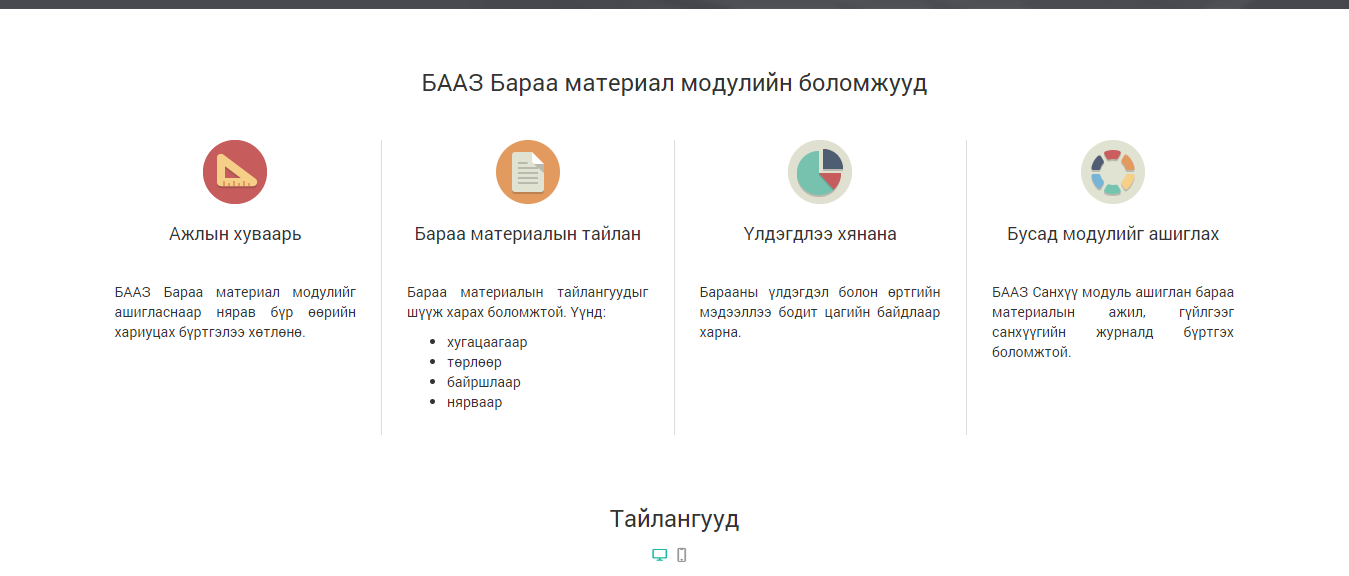
\includegraphics[width=14cm, height=13cm] {Diagrams/k1.png}\\

{\textbf{{Бараа материалын үндсэн бүртгэл}} \par}

Бараа материалыг дараах дарааллаар бүртгэнэ. Үүнд:

{\textbf{Барааны байршил}}



Компаний борлуулах болон дотоод хэрэгцээнд ашиглах зорилгоор эзэмшиж байгаа бараа материалаа хаана хадгалж,борлуулж байгаагаар ангилан харуулсныг барааны байршил гэнэ. Жишээ нь: Агуулах, дэлгүүр гэх мэт

Байршил үүсгэхдээ: Бараа материал > Үндсэн бүртгэл > Барааны байршил>Нэмэх гэсэн дарааллаар хандаж байршил үүсгэнэ. Байршил үүсгэх цонх гарч ирсний дараа бараа материалын нярав, бараа материалын дансуудыг сонгоно.




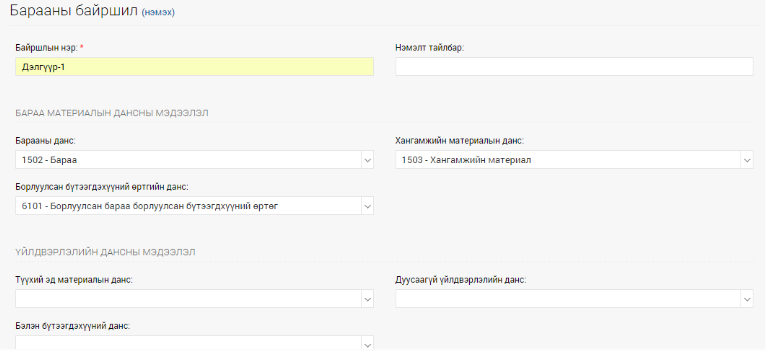
\includegraphics[scale=0.70] {Diagrams/baaz1.png}\\

{\textbf{{БМ-ын ангилал}}
Борлуулах болон дотоод хэрэгцээнд ашиглаж байгаа бараа материалаа төрөл тус бүрээр ангилна. Жишээ нь сүү тараг, жимс жимсгэнэ, хангамж г.м
Бараа материал > Үндсэн бүртгэл > Барааны ангилал > Нэмэх гэсэн дарааллаар хандаж ангилал үүсгэнэ.



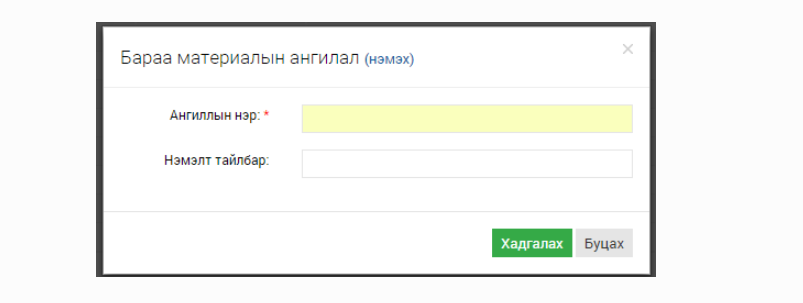
\includegraphics[width=14cm, height=8cm] {Diagrams/f2}

{\textbf{{Бараа материалын эхний үлдэгдэл}}

Бараа материалын эхний үлдэгдлийг 2 янзаар оруулж болно.
Бараа материал > Үндсэн бүртгэл > БМ эхний үлдэгдэл > Засах гэсэн дарааллаар бараа тус бүр лүү орж эхний үлдэгдлээ оруулна. Байршил бүрийн өртөг адил байх бөгөөд байршил бүрийн барааны эхний үлдэгдлийг оруулна.



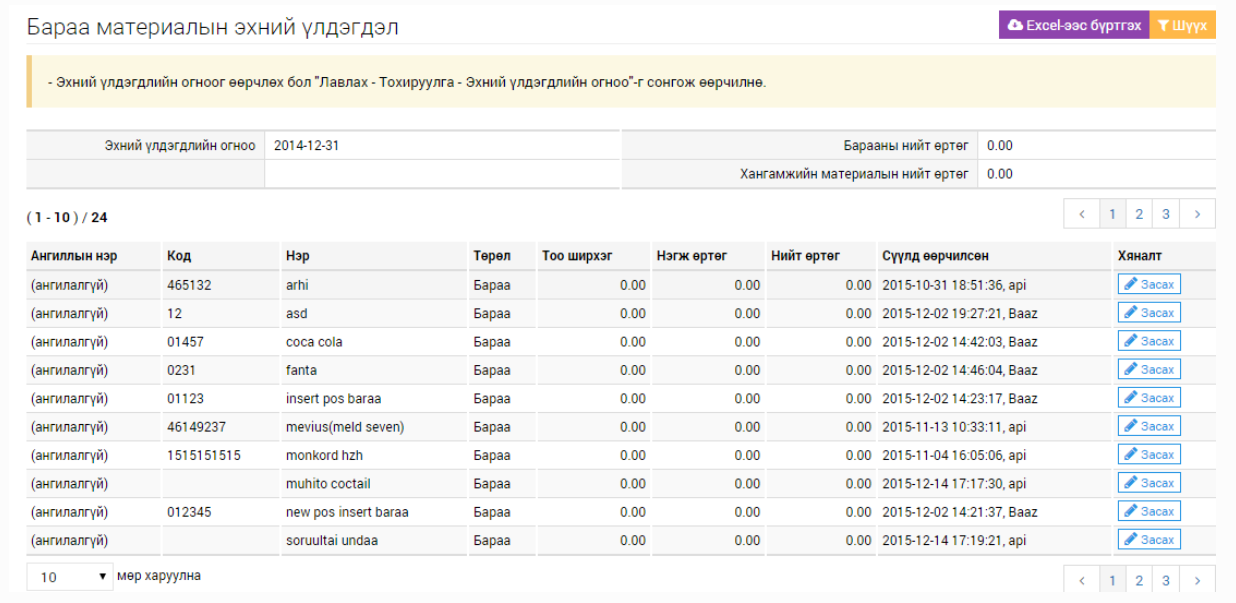
\includegraphics[width=14cm, height=9cm] {Diagrams/f3.png}\\





{\textbf{{Бараа материалын орлого}}
	
	
Худалдан авалт, татан авалт гэсэн 2 хэсгээс бүрдэнэ.



{\textbf{{Худалдан авалт}}
Цаашид худалдах зорилгоор дотоодын бэлтгэн нийлүүлэгчээс бэлнээр болон зээлээр худалдан авсан бараа материалыг худалдан авалтаар бүртгэнэ. Бараа материал > Орлого > Худалдан авалт гэсэн дарааллаар хандана уу.


{\textbf{{Татан авалт}}

Цаашид худалдах зорилгоор импортоор оруулж ирж буй бараа материалыг энд бүртгэнэ. Импортоор оруулж ирж байгаа барааны хувьд бэлтгэх зардлыг нийт дүнд хуваарилах, тоо хэмжээнд хуваарилах гэсэн 2 аргыг ашиглан хуваарилна. Бараа материал > Орлого > Татан авалт гэсэн дарааллаар хандана уу.


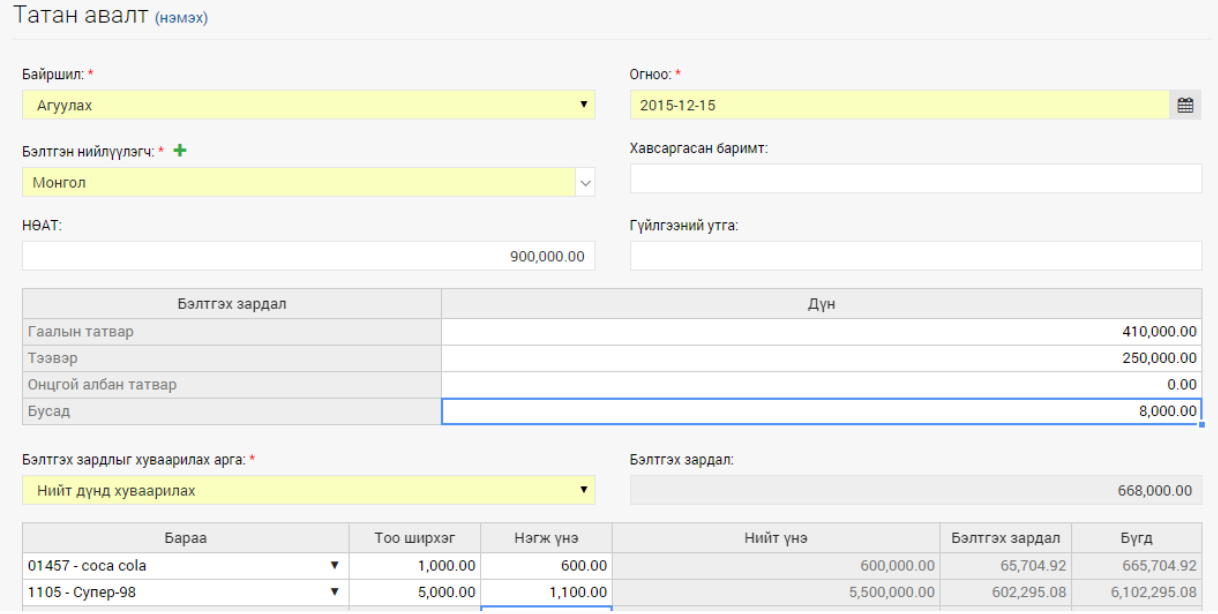
\includegraphics[width=14cm, height=10cm] {Diagrams/f4.png}\\

\begin{itemize}
	\item Odoo erp систем
\end{itemize}

“Odoo ERP“ нь нээлттэй эхэд суурилсан байгууллагын төлөвлөлтийн бүхий л боломжыг агуулсан цогц систем юм. Маш богино хугацаанд маш хурдтайгаар хөгжиж буй систем бөгөөд Odoo ERP нь бизнес менежментийн програм хангамжийн зах зээлд хамгийн өргөн тархацтай системүүдийн нэг болтлоо хөгжиж байна.


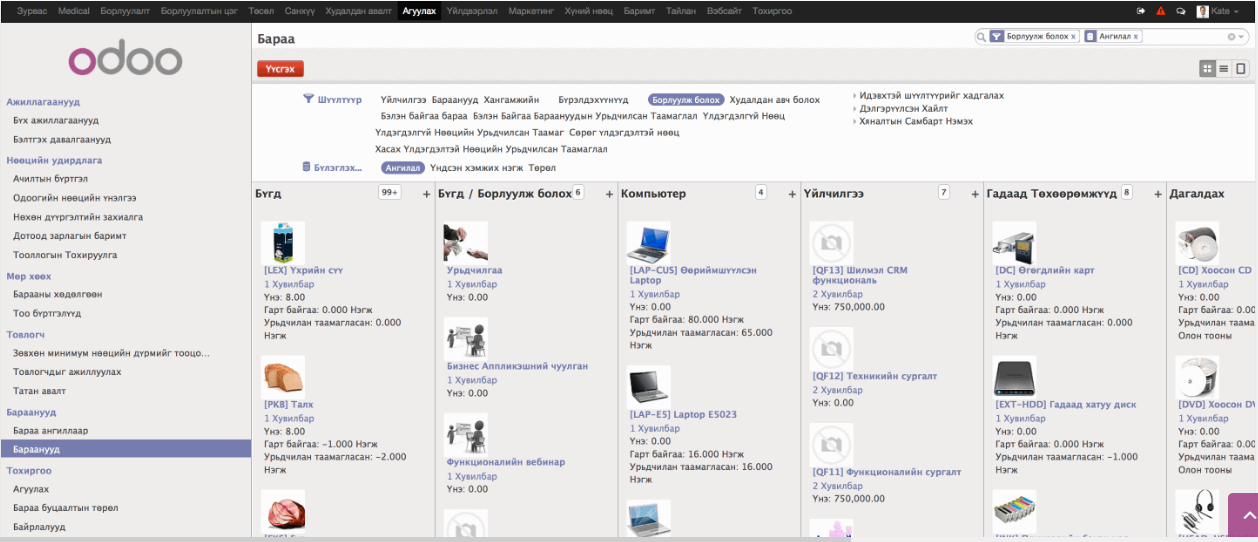
\includegraphics[width=14cm, height=8cm] {Diagrams/f5.png}\\


Агуулах, Бараа материалын модуль

•             Агуулах дахь бараа байрлалуудыг тодорхойлох, удирдах

•             Бараа материалын эргэц болон зохистой үлдэгдлийг удирдах

•             Захиалгад харгалзах багцлалт, савлалтыг удирдах

•             Хүргэлт болон дагалдах баримт, хүргэлтийн зардлыг удирдах

•             Барааны серийн дугаар болон хөдөлгөөний хяналтыг удирдах

•             Автомат нөхөн дүүргэлтийг удирдах

•             Бараа материалын орлого, зарлага

•             Бар код, RFID удирдах

•             Тооллого

•             Буцаалт

•             Актлалт, устгалт

•             Тайлан мэдээ

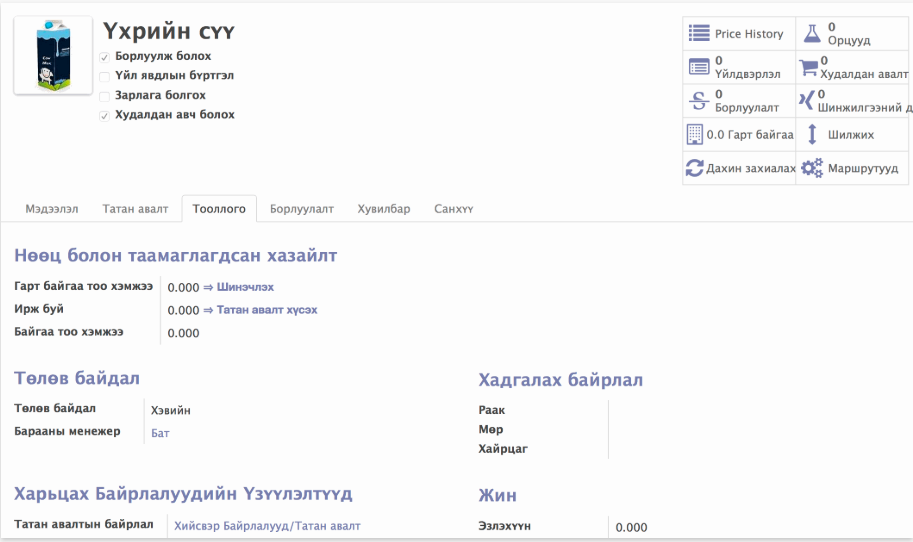
\includegraphics[width=14.5cm, height=12cm] {Diagrams/f6.png}\\
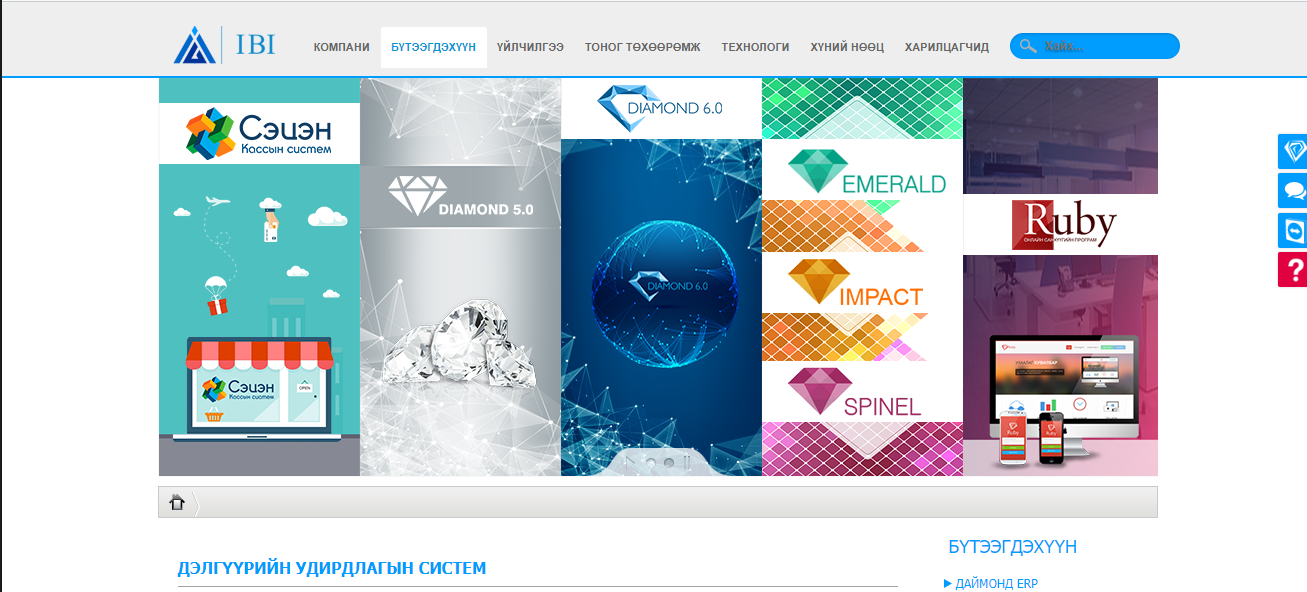
\includegraphics[width=14.5cm, height=10cm] {Diagrams/f7.png}\\
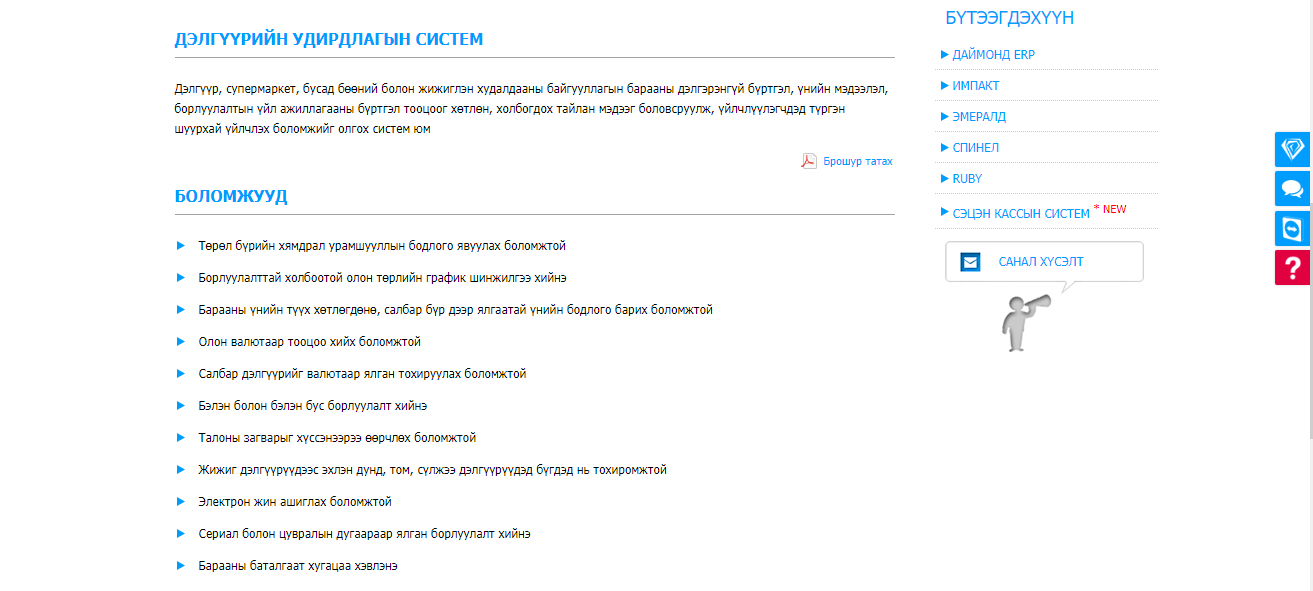
\includegraphics[width=14.5cm, height=12cm] {Diagrams/f8.png}\\
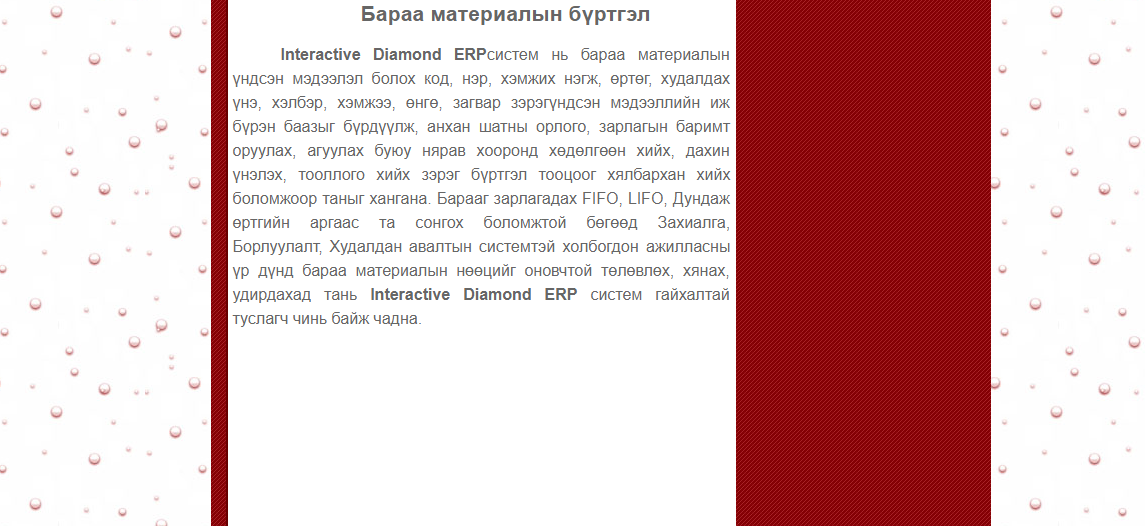
\includegraphics[width=14.5cm, height=10cm] {Diagrams/f9.png}\\
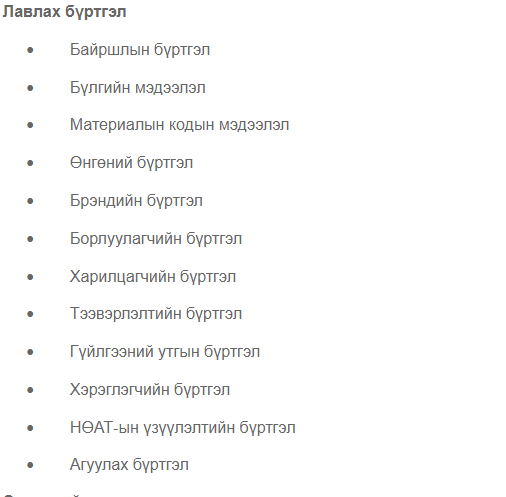
\includegraphics[width=14.5cm, height=12cm] {Diagrams/f10.png}\\
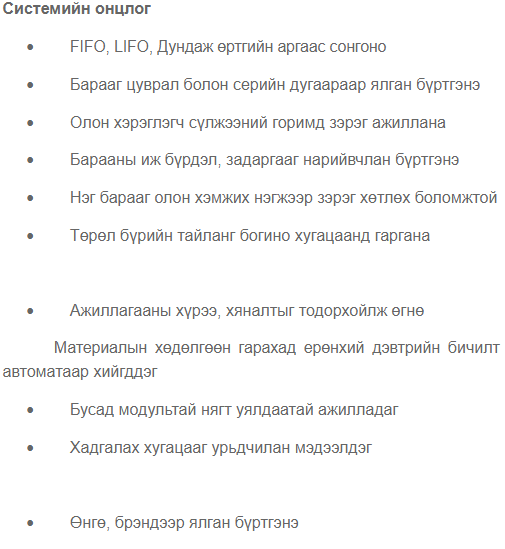
\includegraphics[width=14cm, height=10cm] {Diagrams/f11.png}\\
\subsection{Гадаадын системүүдтэй харьцуулсан судалгаа}
\section{Хууль дүрэм журам}
\qquad Сангийн сайдын 2005 оны 12 дугаар 
сарын 30-ны өдрийн 385 тоот 
тушаалын 1 дүгээр хавсралт


ТӨРИЙН БУС БАЙГУУЛЛАГАД МӨРДӨХ ДАНСНЫ НЭГДСЭН ЖАГСААЛТ

1.1. Энэхүү дансны жагсаалт нь төрийн бус байгууллагын үйл ажиллагааны онцлогийг илэрхийлсэн, нягтлан бодох бүртгэлээр дамжуулан хүлээн авах мэдээллийн хэрэгцээг бүрэн хангахад чиглэгдсэн байна.

1.2. Дансны жагсаалтад дансны агуулга бүрдэх, дансны дугаар хэдэн оронтой байх нь тухайн байгууллагын үйл ажиллагааны цар хүрээ, онцлог, удирдлагын мэдээллийн хэрэгцээнээс хамаарна.

1.3. Дансдыг кодчилах аргачлал нь улсын хэмжээнд нягтлан бодох бүртгэлийн мэдээллийн нэгдсэн систем бүрдүүлэх зорилгод нийцсэн байна.

1.4. Дансны жагсаалт нь балансын болон орлогын тайлангийн дансдуудаас бүрдэнэ.

1.5. Балансын дансдад хөрөнгө, өр төлбөр, хөрөнгийн эх үүсвэрийн дансдууд хамаарах бөгөөд эдгээр  данс тайлангийн үеийн эцэст үлдэгдэлтэй байна.

1.6. Орлого, зардлын дансдууд нь тайлангийн үеийн эцэст орлого, зарлагын нэгдсэн дансанд хаагдана.

1.7. Дансны дугаар нь үйл ажиллагааны онцлог, бүртгэлийн ажиллагааг компьютерээр болон гар аргаар боловсруулж байгаагаас хамааран дөрөв, зургаа, найман оронтой байж болно.

1.8. Энэхүү үлгэрчилсэн зааварт нийцүүлэн үндсэн дансыг туслах дансанд хэрхэн ангилахыг байгууллага өөрөө шийдэж, нягтлан бодох бүртгэлийн бодлогын баримт бичгийг удирдлагаар батлуулж мөрдөнө.
\begin{center}
	А. Баланс данс
\end{center}   
\begin{tabular}{ |p{0.5cm}||p{5cm}|p{1cm}|p{1cm}|p{4.8cm} | }
	\hline
	
	\hline
	Д.д& Дансны бүлэг нэр &Дансны үндсэн ангилал&Дэд ангилал& Дансны дэд ангилалд код өгөх чиглэл\\
	\hline
	&            \textbf{Нэг. Хөрөнгө Эргэлтийн хөрөнгө}
	
	
	Мөнгөн хөрөнгө
	& &  & \\
	1   & Кассад байгаа бэлэн мөнгө    &10&   01 &Төгрөг болон валют түүнчлэн кассын няравын нэрээр, мөнгөний зориулалтаар ангилна.\\
	2&   Харилцахад байгаа мөнгө 
	
	
	& 11   &01 & Данс нээсэн банк болон төсөл, хөтөлбөрийн данс тус бүрээр төгрөг болон валютын гэж ангилна.\\
	3 &Богино хугацаат хөрөнгө оруулалт & 13&  01 &Хадгаламж, түргэн борлогдох үнэт цаасаар хийсэн хөрөнгө оруулалт зэрэг хөрөнгө оруулалтын төрлөөр ангилна.\\
	
	
	\hline
	
	\hline
	
	&           Авлагын данс
	& &  & \\
	4  &Дансны авлага   &12&   01 &Гадаад, дотоодын санхүүжүүлэгч, байгууллага, хувь хүмүүс гэх мэт авлагын төрлөөр ангилна.\\
	5&  Найдваргүй авлагын хасагдуулга 
	
	
	& 12   &.... & \\
	6 &Бусад авлага & 12&  ... &Ажилчин албан хаагчдаас авах авлага, хүүгийн авлага, татварын гэх мэт авлагын төрлөөр ангилна\\
	
	
	\hline
	
	\hline
	
	&          Бараа материал
	& &  & \\
	7  &Бараа материал   &14&   01 &Бараа материал, үнэ бүхий зүйлсийн нэр төрлөөр ангилна.\\
	8& Түлш шатахуун
	
	
	& 14   &.... &Хатуу, шингэн түлш болон эд хариуцагч бүрээр ангилна \\
	9 &Сэлбэг хэрэгсэл
	
	Урьдчилж төлсөн
	
	зардал/тооцоо
	& 14&   &Сэлбэгийн төрөл, эд хариуцагч бүрээр ангилна. \\
	
	10 &Урьдчилж төлсөн зардал/тооцоо
	
	& 18&  01 &Урьдчилж төлсөн зардал, тооцоо болон тэдгээрийн төрлөөр ангилна.\\
	\hline
\end{tabular}


\begin{tabular}{ |p{0.5cm}||p{5cm}|p{1cm}|p{1cm}|p{4.2cm} | }
	
	\hline
	&          
	\textbf{Эргэлтийн бус хөрөнгө}
	
	Үндсэн хөрөнгө
	
	& &  & \\
	11   & Үндсэн хөрөнгө     &20&   01 &Үндсэн хөрөнгийг газар, тавилга, эд хогшил, тээврийн хэрэгсэл гэх мэт төрлөөр нь ангилна.\\
	12&  Үндсэн хөрөнгийн элэгдэл
	
	
	& 20   &... & Үндсэн хөрөнгийн ангилал тус бүрээр элэгдэл байгуулна.\\
	
	
	
	\hline
	
	\hline
	
	&          Биет бус хөрөнгө
	
	
	& &  & \\
	13  &	Биет бус хөрөнгө   &21&   01 &Биет бус хөрөнгийн төрлөөр ангилна.\\
	14&  Хөрөнгө оруулалт
	
	
	& 22   &01 &Хөрөнгө оруулалтын төрлөөр ангилна. \\
	
	
	
	\hline
	
	\hline
	
	&        Хоёр. Өр төлбөр ба байгууллагын өмч
	
	
	Өр төлбөрүүд
	Богино хугацаат өр төлбөр
	
	& &  & \\
	15  &Дансны өглөг   &31&   01 &Бэлтгэн нийлүүлэгч байгууллага, нийгмийн даатгалын шимтгэл, цалингийн өглөг гэх мэт өглөгийн төрлөөр ангилна.\\
	
	16& Татвар, хураамжийн өглөг
	
	
	& 31   &.... &Төрлөөр нь ангилна. \\
	17 &Бусад өглөг
	& 33&   &Өглөг үүссэн байгууллага, хувь хүн тус бүрээр ангилна. \\
	
	18 &Урьдчилж орсон орлого
	
	& 32&  01 &Худалдан авагч байгууллагаас урьдчилж төлсөн орлогыг худалдан авагч бүрээр ангилна.\\
	\hline
	
	19&  Урт хугацаат өр төлбөр
	Урт хугацаат өглөг
	
	
	& 34   &.... &Урт хугацаат өглөгийн төрлөөр ангилна. \\
	\hline
	20& 2.2. Цэвэр хөрөнгө
	Нөөц
	
	
	
	& 41   &01 &Хязгаарлалттай болон хязгаарлалтгүй гэж ангилна. \\
	
	21& Дахин үнэлгээний нэмэгдэл
	Хуримтлагдсан үр дүн
	
	
	
	
	& 42 
	
	44   & & Тайлант үеийн үр дүн ба өмнөх үеийн гэж ангилна. \\
	\hline
\end{tabular}

\vspace{3.6in}
\begin{center}
	Б. ОРЛОГО, ЗАРДЛЫН ДАНС
\end{center}




\begin{tabular}{ |p{0.5cm}||p{5cm}|p{1cm}|p{1cm}|p{4.2cm} | }
	
	\hline
	&          
	\textbf{Нэг. Орлого}
	
	
	
	& &  & \\
	23   & Гишүүдийн татвар     &51&   01 &Гишүүн тус бүрээр ангилна. \\
	24& Хөтөлбөр, төслийн орлого 
	
	
	& 52   &01 &Хэрэгжүүлж буй хөтөлбөр, төсөл тус бүрээр ангилна.\\
	25&Бэлэг, хандив, тусламжийн орлого
	
	
	& 53   &01 &Үйл ажиллагааны зорилго болон хандивлагч тус бүрээр ангилна.\\
	26&Түрээсийн орлого
	
	
	& 54   &01 &Төрлөөр ангилна.\\
	27&Хөрөнгө оруулалтын орлого
	
	
	& 55   &01 &Төрлөөр ангилна.\\
	
	28&Бусад орлого       
	
	
	& 56   &01 &Төрлөөр ангилна.\\
	\hline
	
	\hline
	
	&         \textbf{Хоёр. Зардал} 
	
	
	
	
	
	
	& &  & \\
	29  &	Хандив, тусламжийн зардал   &61&   01 &Тусламж үзүүлсэн байгууллага, хувь хүмүүсээр нь ангилахаас гадна хандив тусламжийг түгээхтэй холбогдон гарсан зардлын төрлөөр нь ангилна.\\
	30&  Хөтөлбөр хэрэгжүүлэх зардал
	
	
	& 62   &01 &Хөтөлбөр тус бүрээр ангилахаас гадна тухайн хөтөлбөрийг хэрэгжүүлэхэд зарцуулсан зардлыг дотор нь зардлын төрлөөр нь ангилна. \\
	31&  Төсөл хэрэгжүүлэх зардал
	
	
	& 63   &01 &Төсөл тус бүрээр ангилахаас гадна төслийн зарцуулалтыг дотор нь зардлын төрлөөр нь ангилна. \\
	32&  Ерөнхий удирдлагын зардал
	
	
	& 70   &01 &Үндсэн ажиллагсдын цалин хөлс, шагнал, урамшуулал, хөнгөлөлт, тэтгэвэр тусламж, томилолтын зардал, тус бүрээр ангилна. \\
	
	\hline

	
\end{tabular}

\vspace{0.1in}
Нягтлан бодох бүртгэлийн үндсэн элементүүд




Нягтлан бодох бүртгэлийн ажил мэргэжил, ажил гүйлгээний хувьцаагсанхүүгийн үйл ажиллагааны нөөцлөлийг эдийн засгийн шинжүүд нягт холбоотой багцзүйл юм.Нягтлан бодох бүртгэлийн элемент нь 5 үндсэн зүйлээс бүрдэнэ.


1.Хөрөнгө санхүү=өр төлбөр+капитал /орлого-зарлага/

2.Эзэмшигчдийн өмч= /орлого-зардал/



Глобал элемент


Тайланг бэлтгэх үзэл баримтлалд мөн л хөрөнгө, өр төлбөр, өмч, орлого, зарлагагэсэн элементүүд орно. Олон улсын стандарт Глобал

Хөрөнгө:


Хөрөнгө гэдэг нь ирээдүйн эдийн засгийн өгөөжийг өгөх өнгөрсөнхөдөлмөрийн үр дүнд бий болсон ирээдүйн баталгаа юм. Өөрөөр хэлбэл ирээдүйн үйлажиллагааны явцад үр өгөөжөө өгөхөөр хүлээгдэж байгаа тухайн бизнесийн өмчлөлдбагтсан үнэ цэнэ бүхий эдийн засгийн нөөцийг хөрөнгө гэж үзнэ. Хөрөнгө заавалөгөөжөө өгнө. Энэ өгөөж янз бүрийн замаар илэрнэ.

1.Хөрөнгө дангаараа эсвэл бусад бүтээгдэхүүнтэй хамтарч байгууллагын борлуулалт

2.Бусад хөрөнгөтэй сольж ашигласнаас өгөөжөө өгнө.

3.Өр төлбөр төлөх замаар өгөөжөө өгнө.

4.Аж ахуйн нэгж, хөрөнгө оруулагчид, нэгжийн эзэд хөрөнгө хуваарилах замаар өгөөжөө өгнө.

Хөрөнгийг үндсэнд нь ашиглагдаж байгаа байдал, өгч байгаа байдал, үзүүлж байгаахалуун тусламжаас хамаарч 2 том бүлэгт хуваана.

1.Эргэлтийн хөрөнгө-хөдөлмөрийн зүйл.

Гол шинж чанар нь үйлдвэрийн үйл ажиллагаанд нэг л удаа оролцоод үйлдэгдэж байгаа бүтээгдэхүүндээ өртгөө бүрэн шингээгээд өгчидөг үнэ өртгөө алдчихдаг. Энэ нь байгууллагын гол амин сүнс юм. Эргэлтийн хөрөнгийн НББ-д бүртгэхэд мөнгө болж хувирах чадварыг буурах дарааллаар байрлуулна.Хөрвөх чадвар хугацаагаар тодорхойлогдно. Хамгийн үнэ цэнэтэй хөрөнгө бол мөнгө юм. Мөнгө болж хөрвөх чадвартай эргэлтийн хөрөнгөд

1. Кассанд байгаа бэлэн мөнгө

2. Харилцах дансан дахь мөнгө

3. Богино хугацаатай хөрөнгө оруулалт

4. Дансны авлага

5. Найдваргүй авлагын нөөц

6. Бекселийн авлага

7. Холбоотой талаас авах авлага


8. Компани хоорондын авлага

9. Түүхий эд материал

10. Дуусгаагүй үйлдвэрлэл

11. Бараа бэлэн бүтээгдэхүүн

12. Хагас боловсруулсан бүтээгдэхүүн

13. Хангамжийн материал

14. Сав баглаа боодол


15. Мал амьтад

16. Урьдчилж төлөх зардал

17. Урьдчилж төлөх тооцоо



Эргэлтийн хөрөнгөөс богино хугацаатай өгөх өрийг хасахад ажлын капитал/карманы зардал/ гарч ирнэ.



2.Эргэлтийн бус хөрөнгө 



Үүний гол шинж чанар нь үйлдвэрлэлийн цикл үед удаан хугацаагаар олон дахин оролцдог. Ингэхдээ хэлбэр дүрс, физик химийн чанараа алдахгүй, бүтээж байгаа бүтээгдэхүүн, үйл ажиллагаандаа өртгөө элэгдснийхээ хэмжээгээр шингээж өгдөг хөрөнгө. Тогтвортой бөгөөд удаан ашиглагдах шинж чанараар нь хөрөнгөө байршуулдаг. Хязгааргүй өгөөжтэй хөрөнгө бол “ГАЗАР” юм. Өөр юу ч байхгүй. 

1. Биет эргэлтийн бус хөрөнгө. Нүдэнд үзэгдэж гарт баригддаг

• Барилга байгууламж, газар


• Барилга байгууламжийн хуримтлагдсан элэгдэл.


• Машин тоног төхөөрөмж, тээврийн хэрэгсэл

• Машин тоног төхөөрмжийн хуримтлагдсан элэгдэл

• Тавилга багаж хэрэгслүүд

• Тавилгад байгуулсан хуримтлагдсан элэгдэл

• Дуусаагүй барилга байгууламж

• Мал амьтад

• Бусад2. 

Биет бус эргэлтийн бус хөрөнгө. 


Нүдэнд үзэгдэхгүй, гарт баригдахгүй гэвчүйлдвэрлэлийн үйл ажиллагаанд идэвхитэй оролцдог.

• Good will’s /нэр хүндийн үнэ цэнэ/

• Патентууд

• Зохиогчийн эрх

• Зохион байгуулалтын зардлууд

• Барааны тэмдэг.

Эргэлтийн ба эргэлтийн бус хөрөнгө дээр хөрөнгө оруулалт, бусад хөрөнгө орно.

Эргэлтийн хөрөнгө+ эргэлтийн бус хөрөнгө+ хөрөнгө оруулалт= Аж Ахуй нэгж,байгууллагын ерөнхий хөрөнгө гарна.

Бүх хөрөнгүүдийн дүнг активын дүн гэнэ. Харин нөгөө эх үүсвэрийг пассив гэж нэрлэнэ.



